Diffusion Models, introduced in 2015 in the paper \href{https://arxiv.org/pdf/1503.03585}{"Deep Unsupervised Learning using Nonequilibrium Thermodynamics" (Sohl-Dickstein et al.)}, are generative models invented at the same time as GANs, but they gained popularity only in 2020. This delay is due to several factors, including computational complexity and the need for more powerful hardware, which has only recently become more accessible and widespread. We now delve into how these models work.

The training of diffusion models can be divided into two main steps:

\begin{enumerate}
    \item \textbf{Forward Diffusion Process ($\mathbf{\textcolor{mypurple}{q(x_{t}|x_{t-1})}}$)}: the contents of an input image are "destroyed" by adding noise over time $t$ until the data distribution becomes a Gaussian.
    \item \textbf{Reverse Diffusion Process ($\mathbf{\textcolor{mypurple}{p_{\theta}(x_{t-1}|x_t)}}$)}: remove noise from the image in order to reconstruct the original image from a Gaussian distribution of noise.
\end{enumerate}

\begin{figure}[!htbp]
    \centering
    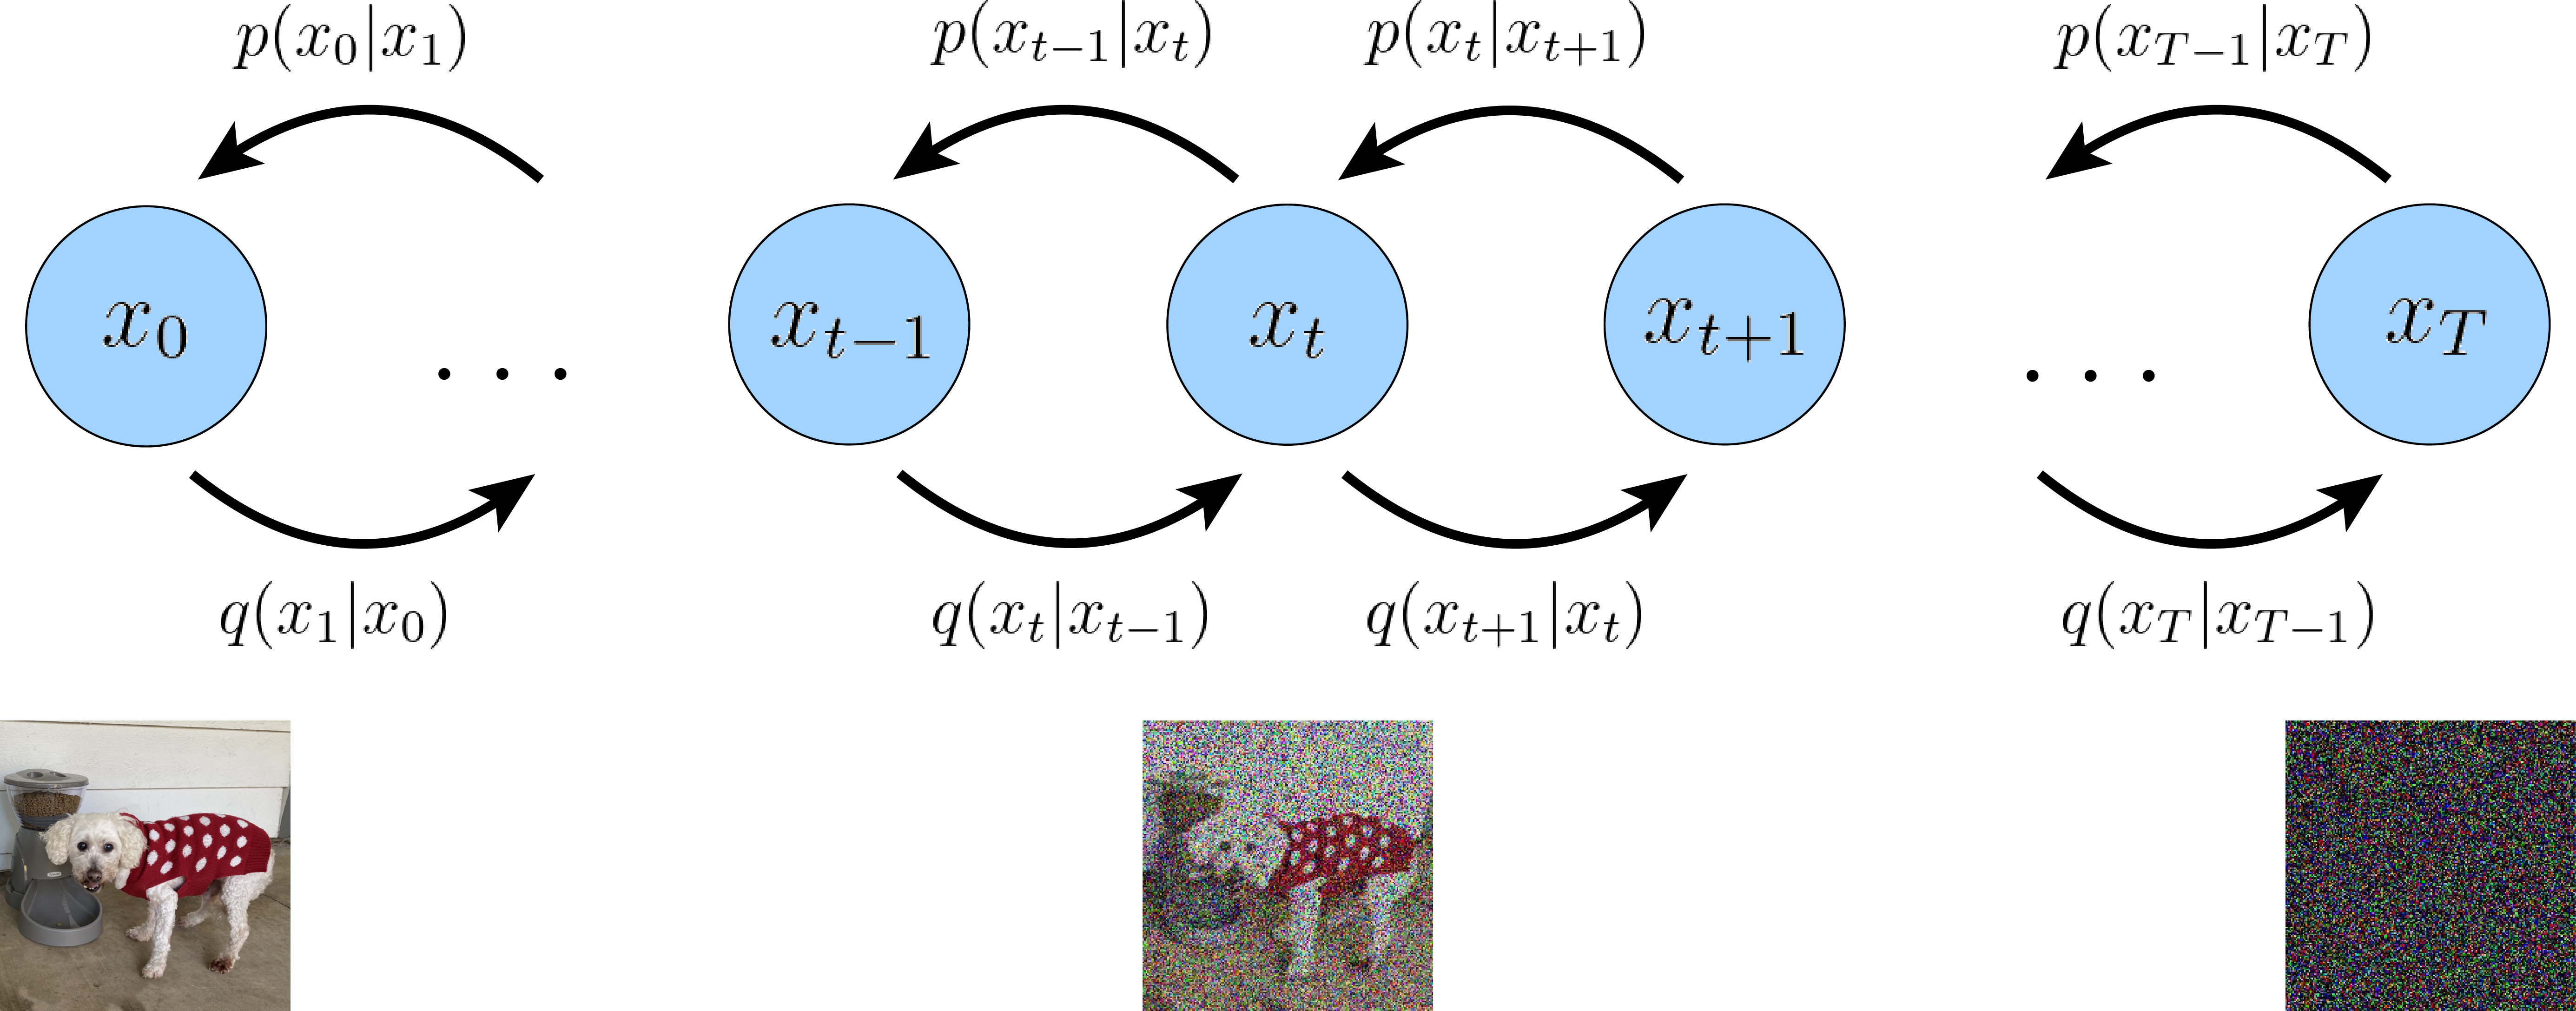
\includegraphics[width=\linewidth]{tikz/chapter10 - Diffusion Models Idea.png}
    \caption{{\color{red}\colorbox{pink}{Tikz TO-DO}} Diffusion Model Idea}
\end{figure}


\section{Forward pass}

To approximate a Gaussian distribution, the added noise is increased slightly at each step ($t$). To obtain a better approximation, the direct diffusion procedure requires \textbf{many iterations} ($T$). However, this involves a trade-off: more steps lead to a better approximation but also increase the computational time required. Therefore, the selection of the number of steps is crucial, since it affects both the quality of the approximation and the computational resources required.

The direct diffusion process gradually adds Gaussian noise to the input image $x_0$ step by step, and there will be $T$ steps in total. The process will produce a sequence of noisy image samples $x_1, \dots, x_T$. \textbf{All intermediate steps are Gaussianly distributed}:

$$q(x_{t}|x_{t-1}) = \mathcal{N}(\sqrt{1-\beta_t}x_{t-1}, \beta_t I)$$

$\beta_t$ represents the \textbf{(small) increase in the noise variance at each time interval} $t$. The formula shows that, at each time, the new Gaussian obtained is centered on the previous sample and rescaled by the variance of the added noise $\beta_t$. \textbf{This makes it possible to approach a zero mean}. If $\beta$ increases, less data are retained when the final Gaussian is obtained ($\sqrt{1-\beta_t}$), and more and more noise is added ($\beta_t I$).

Defining $\alpha_t = (1- \beta_t)$, we can rewrite the formula as:

$$\mathbf{\textcolor{mypurple}{q(x_{t}|x_{t-1})}} = \mathcal{N}(\sqrt{\alpha_t}x_{t-1}, (1-\alpha_t) I)$$

When we sample all steps sequentially, we need to calculate the product of all intermediate random variables:

$$q(x_{1:T}|x_0) = \prod_{t=1}^{T} q(x_t|x_{t-1})$$

Instead of designing an algorithm to compute this iteratively, we can use a \textbf{closed-form formula for a Gaussian process} to directly sample a noisy image (an intermediate step) at a specific time interval $t$ using the \textbf{reparameterization trick}, which we have also seen in VAE:

$$
x_t = \sqrt{\alpha_t}x_{t-1} + \sqrt{(1-\alpha_t)} \epsilon_{t-1}
$$

Where $\epsilon \sim \mathcal{N}(0,1)$, that is, a standard Gaussian random variable.

Then we can expand it recursively by substituting $x_{t-1}$ until we get $x_0$, to get the formula in closed form (\textit{many mathematical derivations have been omitted for your sanity}):

$$x_t = \sqrt{\overline{\alpha}_t}x_{0} + \sqrt{1-\overline{\alpha}_t}\epsilon_0^*$$

Where $\overline{\alpha}_t = \prod_{t=1}^{T}\alpha_t $ and $x_t \sim \mathcal{N}(\sqrt{\overline{\alpha}}_t x_0, (1- \overline{\alpha}_t)I)$.

As we can see, the final formula depends only on the input image $x_0$. This has a significant implication: \textbf{it allows us to directly sample $x_t$ at any time interval}, making the direct diffusion process much faster since we do not have to compute the entire product of all time intervals. The significance is that we can sample any intermediate $x_t$ simply by multiplying all $\alpha_{t}$ along the way. \textbf{As $t$ gets closer to $T$, i.e., after many steps, we eventually get an (almost certainly) Gaussian distribution.}


\section{Reverse pass}


So far, we have seen how to destroy all image information using efficient transformations, but this procedure \textbf{does not involve any training}. What we lack is an understanding of how the model can generate a sample from this final Gaussian distribution. In particular, \textit{how does the model learn to reverse the process and transform the noise back into the original data distribution?}

Unlike the forward process, we cannot use $p(x_{t-1}|x_t)$ to reverse the noise because the \textbf{\textcolor{myred}{denominator $p(x_t)$}} and the \textbf{\textcolor{myred}{marginal distribution of an intermediate step $p(x_{t-1})$}} are \textbf{\textcolor{myred}{intractable}}:

$$p(x_{t-1}|x_t) = \frac{p(x_t|x_{t-1})\textcolor{myred}{p(x_{t-1})}}{\textcolor{myred}{p(x_t)}}$$

Therefore, we need to train a neural network $p_{\theta}(x_{t-1}|x_{t})$  to approximate the inverse process $p(x_{t-1}|x_t)$,  i.e., to approximate the posterior distribution (\textit{...sounds familiar?}). The approximation $p_{\theta}(x_{t-1}|x_t)$ follows a normal distribution (\textbf{remember that the inverse of a Gaussian process is still a Gaussian distribution}), and the \textbf{neural network learns/models only the parameter $\mu_{\theta}$ of the inverse Gaussian process}, since the \textbf{\textcolor{mygreen}{variance is fixed}}, i.e., it is shared among the intermediate inverse steps:

$$\mathbf{\textcolor{mypurple}{p_{\theta}(x_{t-1}|x_t)}} = \mathcal{N}(\mu_{\theta}(x_t, t), \textcolor{mygreen}{\Sigma_t})$$

\begin{remark}{accent}{accent!10}
As you may have already realized, diffusion models can be seen as a \textbf{special case of (hierarchical) VAE}, but:
\begin{itemize}
    \item The encoder is fixed (it is the forward process).
    \item The latent variables have the same dimensionality as the data.
    \item The same model is applied to different time intervals.
\end{itemize}
\end{remark}

With this approach, instead of directly optimizing the intractable loss function, we can \textbf{optimize the Variational Lower Bound}. Eventually, the neural network can be trained with \textbf{ELBO (Evidence Lower Bound)}:

$$
\mathcal{L} = \textcolor{myorange}{\mathbb{E}_{q(x_1 | x_0)} \left[ \log p_{\theta}(x_0 | x_1) \right]} - \textcolor{myblue}{\sum_{t=2}^{T} \mathbb{E}_{q(x_t | x_0)} \left[ D_{KL} \left[ q(x_{t-1} | x_t, x_0) \| p_{\theta}(x_{t-1} | x_t) \right] \right]}
$$

The first term represents a \textbf{\textcolor{myorange}{boundary condition}} and the second term is a \textbf{\textcolor{myblue}{KL divergence at every other step}}.

Using this formula, we perform some mathematical steps and derivations: calculate the closed form for the second term, simplify the closed form by focusing directly on the divergence in the added noise, rewrite the first term by defining it through the added noise, define the lower bound of the log-verosimilarity of a sample, and use the Monte Carlo approximation to not compute all the time steps of all the samples. \textit{Fortunately for you, we will not see all these steps in detail but only the final closed formula that is used for the inverse process.}

The inverse process, which removes the added noise, is described by the following closed formula (\textit{oh, of course we are also using the reparameterization trick}):

$$
x_{t-1} = \frac{1}{\sqrt{\alpha_t}} \left( x_t - \frac{\beta_t}{\sqrt{1 - \overline{\alpha_t}}} \epsilon_{\theta}(x_t, t) \right) + \sigma_t z
$$

We have finally obtained an efficient formula that achieves the training goal: \textbf{an iterative process that allows the model to transform noisy data into clean data by progressively removing estimated noise}.


\section{Generative Trilemma}

So far, we have examined three types of generative models: the GANs, VAEs, and diffusion models. Below is an image that briefly summarizes their different architectures:

\begin{figure}[!htbp]
    \centering
    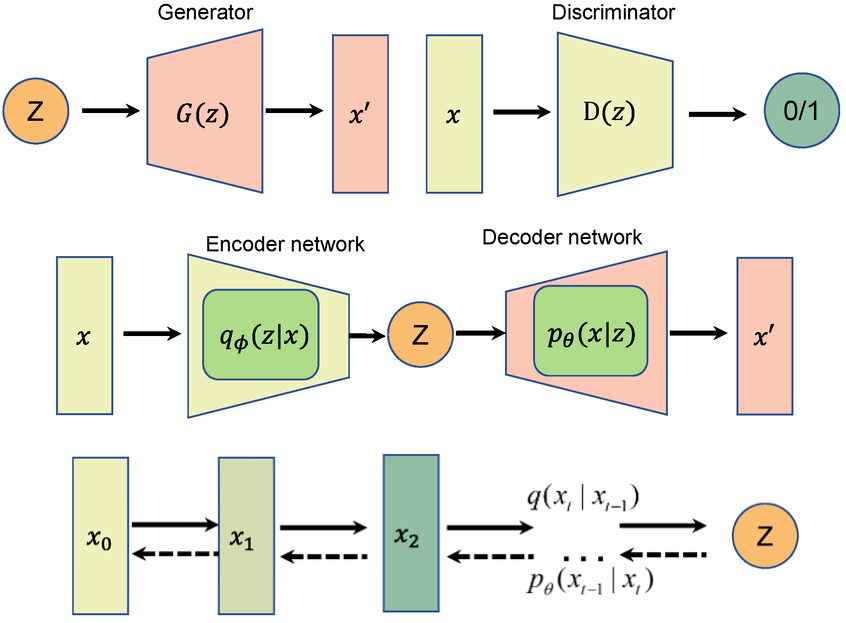
\includegraphics[width=0.7\linewidth]{tikz/chapter10 - Generative Models Comparison.png}
    \caption{{\color{red}\colorbox{pink}{Tikz TO-DO}} Generative Models Comparison}
\end{figure}



In NVIDIA's paper \href{https://arxiv.org/pdf/2112.07804}{"Tackling the Generative Learning Trilemma with Denoising Diffusion GANs" (Vahdat et al.)}, the authors state that, in the context of generative models, there is a trilemma based on three properties: \textbf{Fast Sampling}, \textbf{Diversity} (Mode Coverage) and \textbf{High Sample Quality}. Interestingly, our three types of generative models excel in different combinations of these properties:

\begin{itemize}
    \item \textbf{VAEs}: Fast Sampling and Diversity.
    \item \textbf{GANs}: Fast Sampling and high Quality.
    \item \textbf{Diffusion Models}: High Quality and Diversity.
\end{itemize}

Recently, diffusion models have made significant progress in fast sampling, trying to balance all three properties.

\begin{figure}[H]
    \centering
    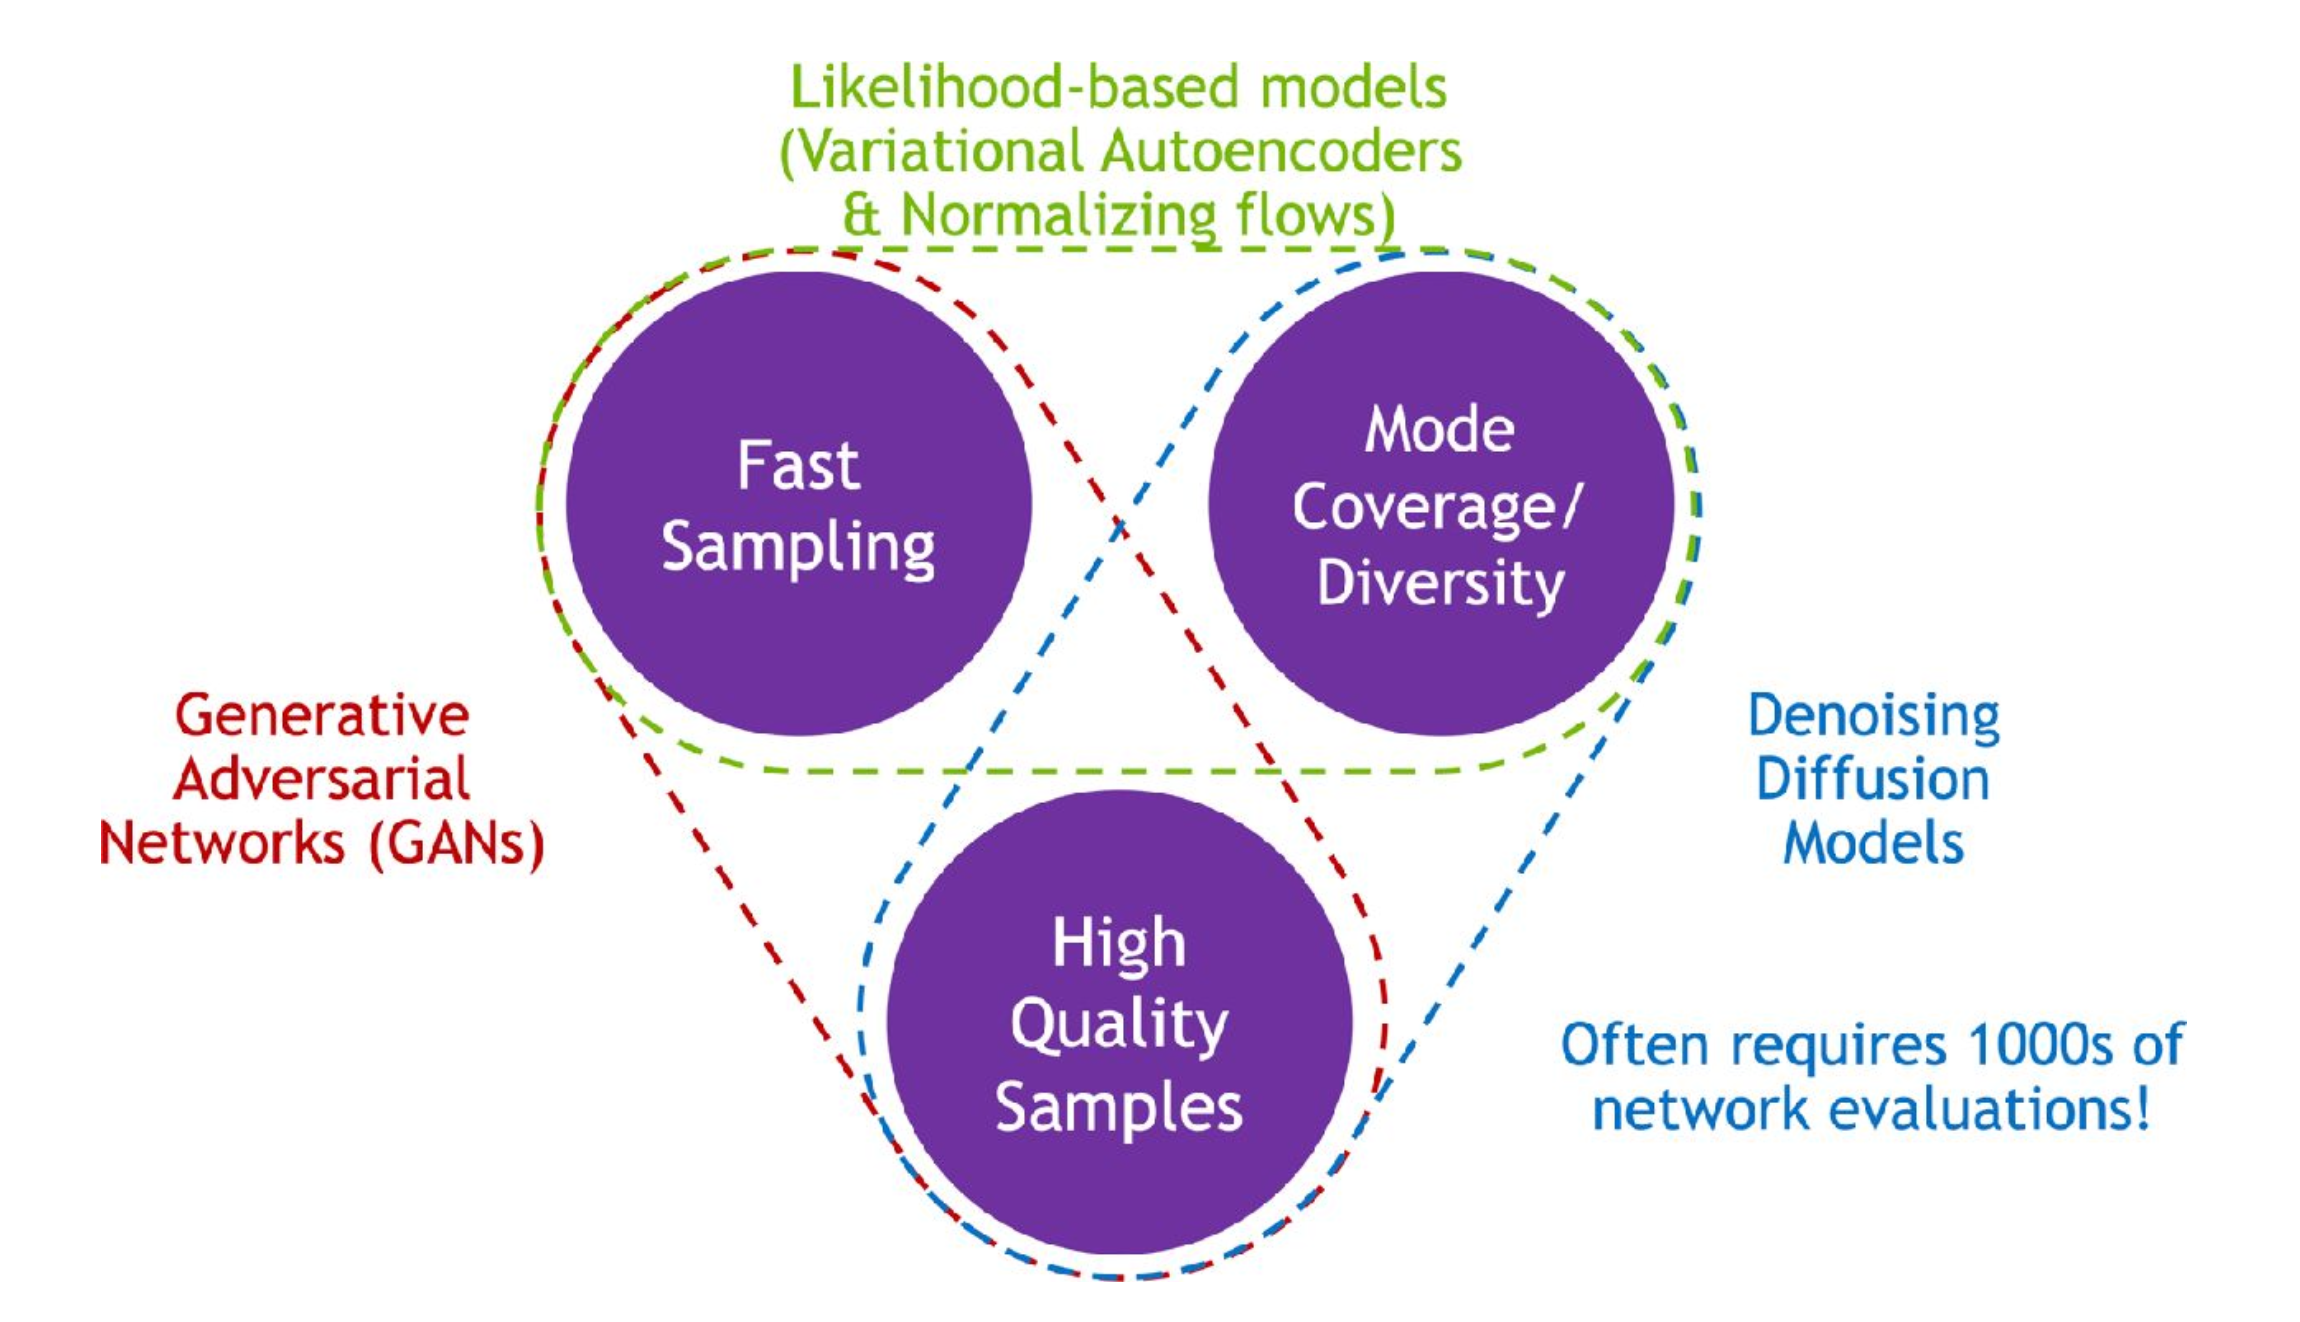
\includegraphics[width=0.8\linewidth]{tikz/chapter10 - Generative Trilemma.png}
    \caption{Generative Trilemma}
\end{figure}

\section{Stochastic Equation and Denoising Score Matching}

In this very short section we will give an \underline{high-level} overview two fundamental aspects of training diffusion models.

In the forward diffusion process, noise is added to the original image at each step. This process can be described by a \textbf{stochastic equation that separates the effect of noise into two components}: one representing \textbf{average change} and one representing \textbf{random variation}. For the reverse process, which aims to reconstruct the original image, these two components are used to guide the model in removing the noise.

Training a diffusion model is based on \textbf{Denoising Score Matching}, which aims to minimize the difference between the noise added and the noise estimated by the neural network. This approach allows the model to refine its ability to interpolate between latent spaces, resulting in continuous and semantically meaningful changes in the data.

\section{Network Architecture and Text Conditioning}

The network architecture used in diffusion models can vary, but is often inspired by established models such as PIX2PIX. In this configuration, \textbf{temporal information is embedded via Fourier features}, which can be represented by sinusoidal (sine and cosine) functions, similar to positional embedding. These features help to encode time more expressively. 

For images, the \textbf{U-Net architecture, with the addition of attention mechanisms, is commonly employed to preserve and reconstruct complex spatial details}. In addition, Vision Transformers (ViTs) can be used to exploit self-attention mechanisms, enhancing the model's ability to capture complex patterns and relationships in images. The choice of how to incorporate temporal features and the underlying network is relatively free, with no stringent theoretical constraints.

\begin{figure}[!htbp]
    \centering
    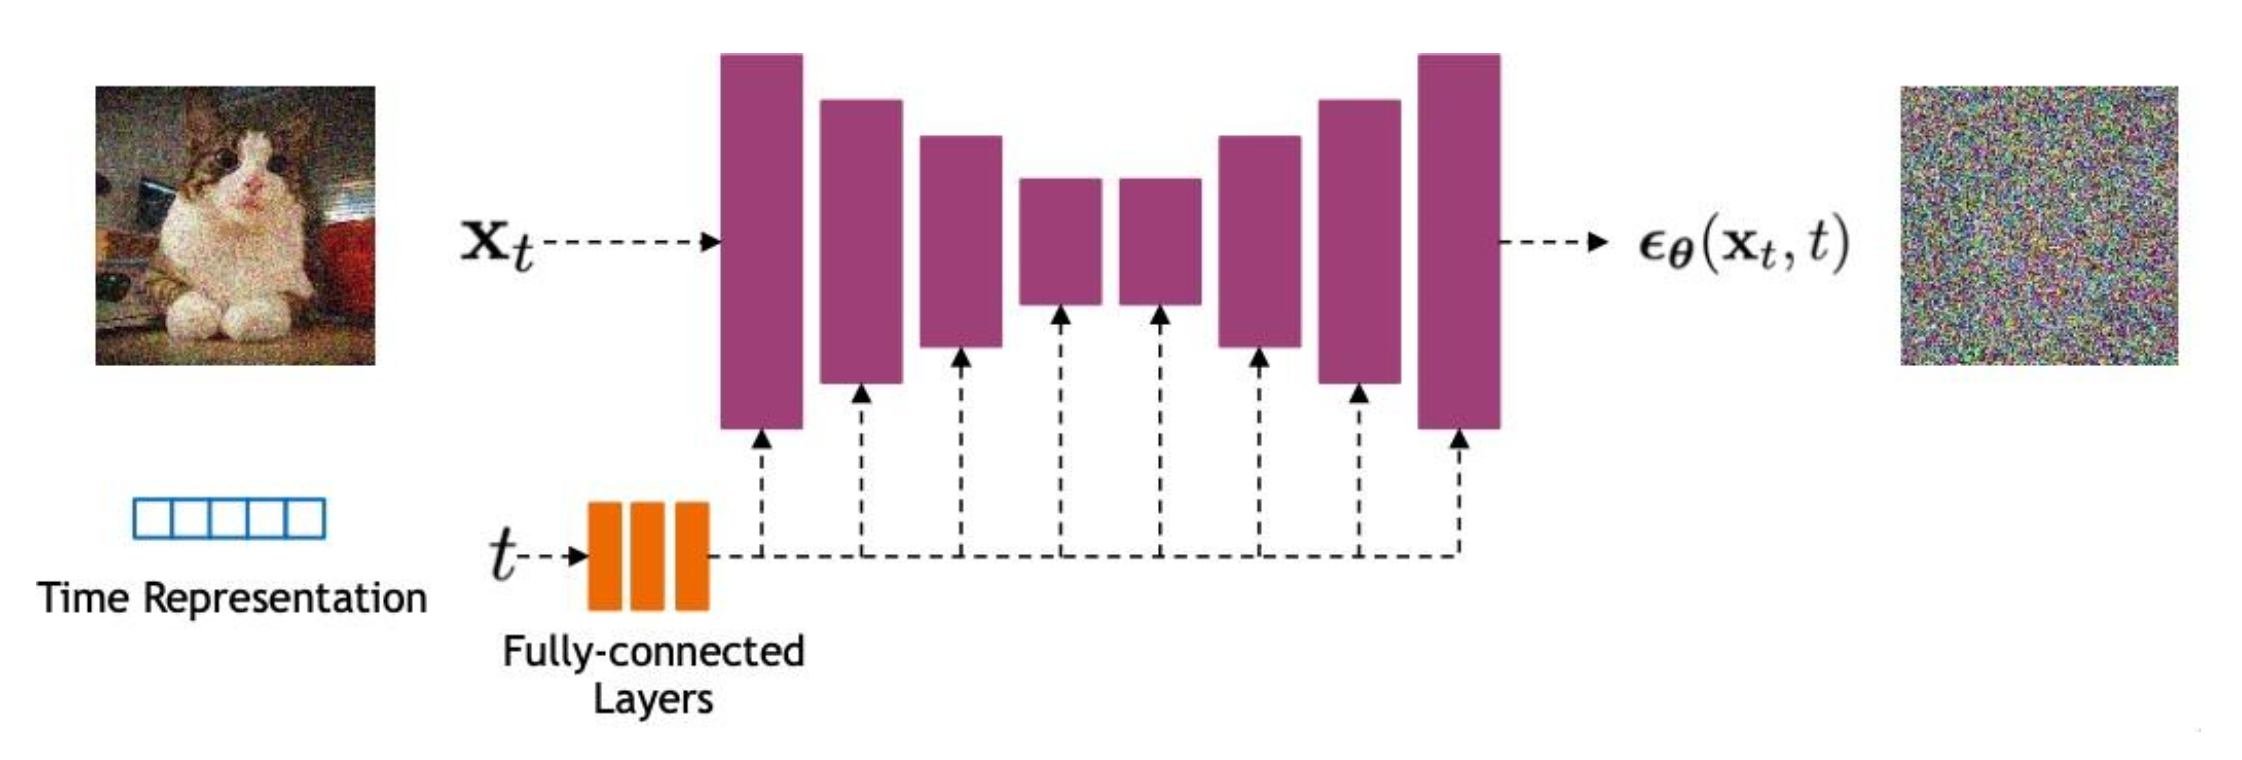
\includegraphics[width=\linewidth]{tikz/chapter10 - Diffusion Models Network Architecture.png}
    \caption{{\color{red}\colorbox{pink}{Tikz TO-DO}} Diffusion Model Architecture Example}
\end{figure}

\textit{But how can we guide diffusion models to generate text-based images?} The \textbf{Text Conditioning} in diffusion models uses textual information to influence image generation. Here is a (highly synthesized) summary of the process:

\begin{itemize}
    \item \textbf{Textual Embeddings:} Textual descriptions are converted into numerical vectors using embedding models such as CLIP, which capture the meaning of the text. Textual embeddings are integrated into the diffusion model, guiding the generation of the image to reflect the provided description.
    
    \item \textbf{Training:} The model is trained on text and image pairs, learning to generate images that match the text descriptions. The goal is to minimize the difference between the generated image and the target image based on the text.
\end{itemize}

\section{Stable Diffusion}

At the end of this chapter on diffusion models, it is important to mention a significant advance in the field: \textbf{Stable Diffusion}, described in the article \href{https://arxiv.org/pdf/2112.10752}{"High-Resolution Image Synthesis with Latent Diffusion Models" (Rombach et al.)}. This approach represents an evolution from traditional diffusion models, introducing some key innovations. Here are the main ones:

\begin{itemize}
    \item \textbf{Latent Space:} Instead of applying the diffusion process directly on high-resolution images, Stable Diffusion operates in a compressed latent space. This latent space is represented by a \textbf{low-dimensional encoding of the images}, obtained through an encoder. Diffusion takes place on these latent representations, significantly \textbf{reducing computational costs and making the process more efficient}. Next, a decoder reconstructs the original images from the latent space.

    \item \textbf{Denoising U-Net:} In the reverse process, Stable Diffusion uses a U-Net for denoising. This network is designed to remove noise from latent representations and restore the original images with high quality. The U-Net model is \textbf{equipped with attention mechanisms} that enhance the model's ability to capture and reconstruct complex image details.

    \item \textbf{Conditioning Space:} Stable Diffusion can also include additional conditions, such as text or other semantic information, to \textbf{guide image generation}. This conditioning space allows images to be tailored to specific textual descriptions or other constraints, increasing the model's versatility in synthesizing visual content.
\end{itemize}

\begin{figure}[!htbp]
    \centering
    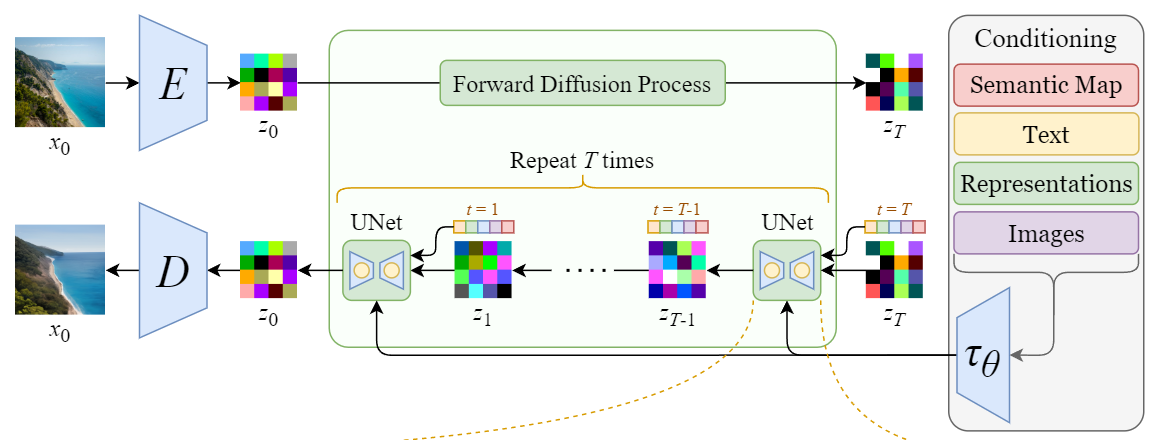
\includegraphics[width=\linewidth]{tikz/chapter10 - Stable Diffusion Architecture.png}
    \caption{{\color{red}\colorbox{pink}{Tikz TO-DO}} Stable Diffusion Architecture}
\end{figure}

This approach enables practical challenges in high-resolution image synthesis, making visual content generation more affordable and scalable.
